\chapter{Experiment and Results}\label{ch:5}

\section{Questionnaires}

In the proposed framework, there are several components we have to validate in order to answer our research questions.
The following list explains the targets to validate, and Figure 5.1 indicates where the targets are located in our proposed framework.

\begin{quote}
  \begin{itemize}
    \item T1: Motivation to access the campus by location-based AR contents
    \item T2: Change in images of the campus by location-based AR contents
    \item T3: Motivation to access the campus by co-creation process
    \item T4: Change in images of the campus by co-creation process
    \item T5: Motivation to access the campus by interaction between users
    \item T6: Change in images of the campus by interaction between users
  \end{itemize}
\end{quote}

\begin{figure}[ht]
  \centering
  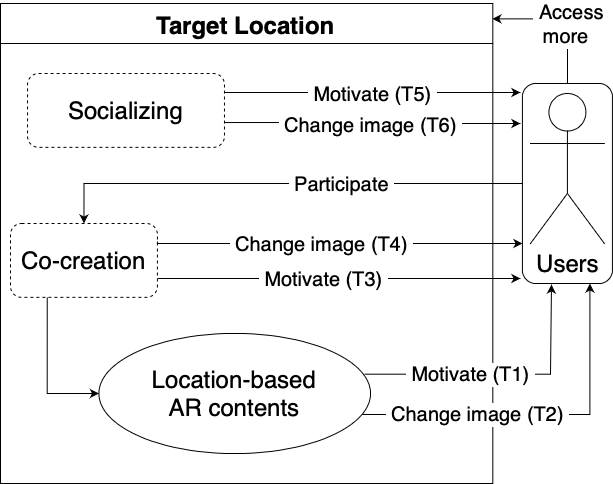
\includegraphics[width=0.8\columnwidth]{resources/5_experiment_and_results/proposed_framework_with_validate_targets.png}
    \caption{Proposed framework and targets to validate}
\end{figure}

Then we designed four questionnaires for the validation, and each of them holds a topic:

\begin{quote}
  \begin{enumerate}
    \item Viewing location-based AR contents, the graffiti, in the campus
    \item Creating location-based AR contents, the graffiti, in the campus
    \item Interactions with other users
    \item Overall experience of using the prototype
  \end{enumerate}
\end{quote}

In each questionnaire, we asked questions about how the experience of the topic during the experiment changes one's motivation to access the campus, image of the campus in one's mind, one's preference between the prototype or a similar one but playable at home.
Questions in Questionnaire 1 are prepared for validating T1 and T2, Questionnaire 2 for T3 and T4, Questionnaire 3 for T5 and T6, topic 4 for the whole framwork.
For Questionnaire 1, 2 and 4, we also asked questions about participants' feeling of presence to check its relevance to the questionnaire's topic, while for topic 3 we asked questions about awareness of other users' existence and interaction.
In the measurement of motivation, we adopted Situational Motivation Scale (SIMS) \cite{guay_vallerand_blanchard_2000} in this study.

\section{Experiment}

At first, we conducted a preliminary survey with 3 participants trying the prototype in Waseda University Nishi-Waseda Campus for one week.
3 participants gave us positive responses about their motivation to access campus after experiencing the prototype.
We also improved the app based on their feedbacks, such as adding features that allow users to review/edit/delete their own graffiti.
The experinemt lasted for 2 weeks. 14 males and 2 females participated,
and they are asked to use the prototype freely in the same campus at least twice a week.
Before the experiment, we asked participants about their frequencies of accessing the campus and the images of campus in their mind before and after the pandemic started spreading,
in order to understand how much impact the pandemic brought on each participant.
Instruction of using the prototype was also distributed before the experiment.
2 weeks later, after the experiment finished, participants were required to answer the questionnaires introduced in Section 5.2.

\section{Results}
\subsection{Motivations}

\begin{table}[h]
  \begin{tabular}{l || R{4cm} | R{3cm} | R{2.5cm}}
    \hline
    \rowcolor{lightgray}
          & \multicolumn{1}{c |}{Intrinsic motivation (IM)} & \multicolumn{1}{c |}{Amotivation (AM)} & \multicolumn{1}{c}{IM - AM}  \\
    \hline
    Mean   & 4.3906 & 2.7500 & 1.6406  \\
    Median & 4.3750 & 3.0000 & 1.6250  \\
    Min    & 3.0000 & 1.0000 & -1.5000 \\
    Max    & 6.0000 & 4.5000 & 5.0000  \\
    SD     & 0.7636 & 1.0124 & 1.5916  \\
    \hline
  \end{tabular}
  \caption{Measurement results with SIMS: Motivation to access campus influenced by viewing location-based AR contents}
    \label{table:1}
\end{table}

\begin{table}[h]
  \begin{tabular}{l || R{4cm} | R{3cm} | R{2.5cm}}
    \hline
    \rowcolor{lightgray}
          & \multicolumn{1}{c |}{Intrinsic motivation (IM)} & \multicolumn{1}{c |}{Amotivation (AM)} & \multicolumn{1}{c}{IM - AM}  \\
    \hline
    Mean   & 4.4833 & 2.5167 & 1.9667  \\
    Median & 4.2500 & 2.5000 & 2.0000  \\
    Min    & 3.0000 & 1.0000 & -1.5000 \\
    Max    & 6.0000 & 4.5000 & 5.0000  \\
    SD     & 0.8044 & 1.0021 & 1.6767  \\
    \hline
  \end{tabular}
  \caption{Measurement results with SIMS: Motivation to access campus influenced by participation in co-creation}
    \label{table:2}
\end{table}

\begin{table}[h]
  \begin{tabular}{l || R{4cm} | R{3cm} | R{2.5cm}}
    \hline
    \rowcolor{lightgray}
          & \multicolumn{1}{c |}{Intrinsic motivation (IM)} & \multicolumn{1}{c |}{Amotivation (AM)} & \multicolumn{1}{c}{IM - AM}  \\
    \hline
    Mean   & 4.3833 & 2.5833 & 1.7200  \\
    Median & 4.7500 & 2.0000 & 1.8000  \\
    Min    & 2.0000 & 1.0000 & -2.0000 \\
    Max    & 6.0000 & 5.0000 & 5.0000  \\
    SD     & 1.1135 & 1.1286 & 2.0743  \\
    \hline
  \end{tabular}
  \caption{Measurement results with SIMS: Motivation to access campus influenced by interaction with other users}
    \label{table:3}
\end{table}

\begin{table}[h]
  \begin{tabular}{l || R{4cm} | R{3cm} | R{2.5cm}}
    \hline
    \rowcolor{lightgray}
          & \multicolumn{1}{c |}{Intrinsic motivation (IM)} & \multicolumn{1}{c |}{Amotivation (AM)} & \multicolumn{1}{c}{IM - AM}  \\
    \hline
    Mean   & 4.5469 & 2.5313 & 2.0156  \\
    Median & 4.6250 & 2.2500 & 2.6250  \\
    Min    & 3.0000 & 1.0000 & -2.0000 \\
    Max    & 6.0000 & 5.0000 & 5.0000  \\
    SD     & 0.8328 & 1.0950 & 1.8108  \\
    \hline
  \end{tabular}
  \caption{Measurement results with SIMS: Motivation to access campus influenced by overall experience of the prototype}
    \label{table:4}
\end{table}

\subsection{Image of Campus}

\subsection{User-user Interaction}

\subsection{Revelance of Feeling of Presence}